\section{Homepage}\label{sec:homepage}
A short description of each of the functionalities is available for the user on the homepage of the application, seen in \Cref{fig:figure3.1}.
Nevertheless, they will be explained here as well.

The first step for creating the representation is to enter the cities the artist lived in, using a map. The map already shows all the available cities
from the previously entered artists. After entering the cities, the artist's information is entered. Finally, external events like exhibitions and historic events
can be entered, so that they can be represented in the cube as well.

Each functionality will be described in detail in the following sections.

\clearpage

\begin{figure}[hbt!]
    \begin{center}
        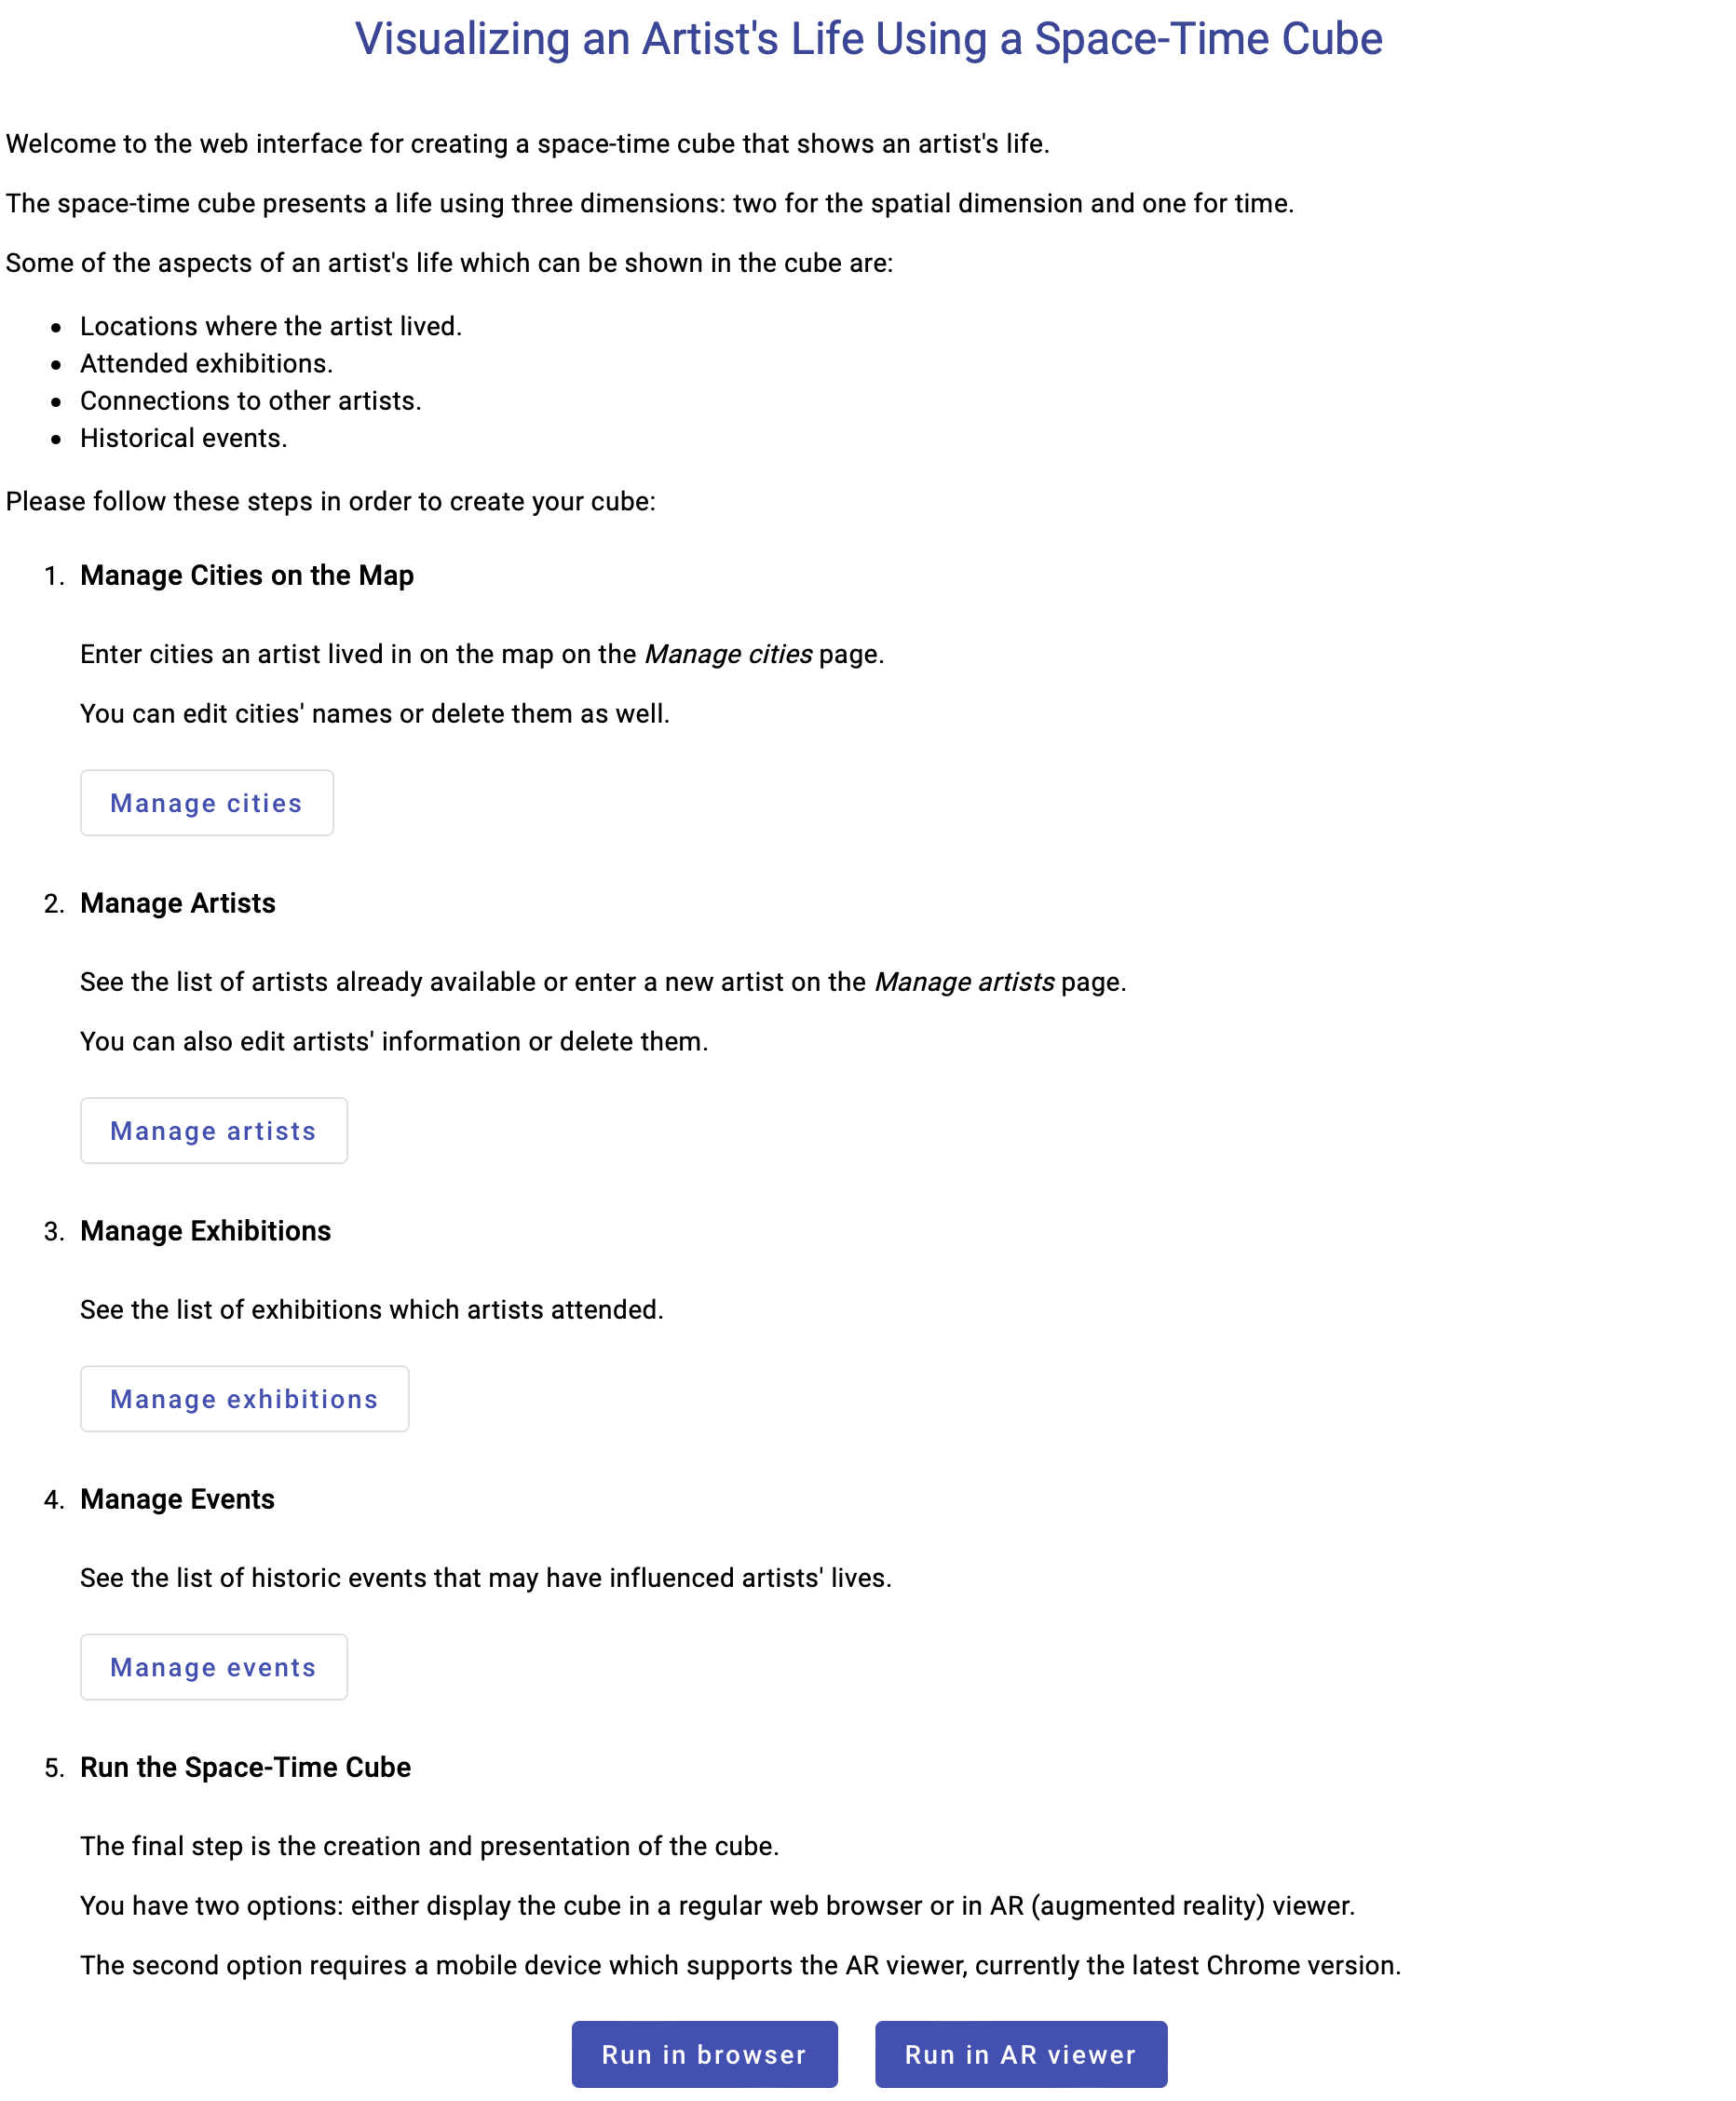
\includegraphics[width=\textwidth]{graphics/3-implementation/1}
    \end{center}
    \caption{Homepage view of the web application}
    \label{fig:figure3.1}
\end{figure}